% \begin{savequote}[75mm]
% This is some random quote to start off the chapter.
% \qauthor{Firstname lastname}
% \end{savequote}

\chapter{Hawkes Processes with Latent Network Structure}
\label{chap:three}

Networks are fundamental models for complex systems, enabling us to
reason about systems by studying the relationships between their
parts.
As we discussed in Chapter~\ref{chap:one}, networks are employed in a myriad of ways throughout
neuroscience.  Whether they represent synapses in the human
connectome, systems-level interactions in brain circuits, pairwise
correlations in fMRI recordings, or coupling in theoretical models,
networks abstract away the messy details of systems.  A network consists of nodes, which
may represent neurons, populations, voxels, etc., depending on the application.
Connecting these nodes is a set of edges, 
which represent interactions between  pairs of nodes, like the effect
of one neuron's spikes on the subsequent activity of its downstream
neighbors.  By reducing a system to a network of nodes and edges,
we create a simplified object for analysis.

%Representing these systems as networks facilitates a number of
%analyses. 
A great deal can be learned by considering simple network properties
like the average number of connections per node, or higher order
statistics like ``betweenness'' and the number of connected triangles
\cite{bullmore2009complex}.  Some network analyses involve
probabilistic modeling.  For example, we may look for clusters or
features of nodes that have similar patterns of connectivity.  Other
analyses are more supervised in nature; in a ``link prediction'' task
we want to predict whether or not a pair of nodes is connected, given
partial observations of the network.
%In some cases,
% we wish to classify networks recorded from healthy and diseased patients. 
 Traditionally, network analysis has focused on \emph{explicit
   network} problems in which the network itself is considered to be
 the observed data.  That is, the nodes are and edges are considered
 known. A rich literature has arisen in recent years for applying
 statistical machine learning models to this type of problem, e.g.,
 \citet{Liben-2007,Hoff-2008,Goldenberg-2010}.

In practice, however, we are often confronted with \emph{implicit
  networks} that cannot be observed directly, but about which we wish
to perform analysis.  In an implicit network, the nodes or edges of
the network may not be directly observed, but the graph structure may
be inferred from noisy emissions.  These noisy observations are
assumed to have been generated according to an underlying model that
respects the latent network structure.

For example, in connectomics problems the network must be inferred
from noisy electron microscopy images; in spike train modeling the
network must be inferred from weak anatomical evidence and noisy
measurements of population activity; and in fMRI experiments, the
network is derived from noisy BOLD responses.  In both cases, if we
knew the underlying network (i.e.  if we knew how the nodes were
connected), we could assign a likelihood to the observed electron
microscopy images or to the measured activity. By combining this
likelihood with a prior distribution that reflects our intuitions
about the network structure, we can construct a probabilistic model to
tackle these implicit network problems.


In this chapter, we consider the case where our observations come in
the form of neural spike trains, and our intuition is that a spike on
one neuron will influence the activity of downstream neurons.  We formalize
this with a probabilistic model based on mutually interacting point
processes.  Specifically, we combine the Hawkes process
\cite{Hawkes-1971} with hierarchical prior distributions on the network.  This
combination allows us to reason about properties of neurons that govern
network structure, which in turn governs the dynamics of activity via
a Hawkes process. Inference
in the resulting model is done with Markov chain Monte Carlo by leveraging
an elegant data augmentation scheme that allows efficient parallelism.

Figure~\ref{fig:network_hawkes} illustrates the components of the
probabilistic model. At the highest level, we have a network of
neurons.  The pattern of connectivity in the network may be governed
by latent variables like cell types and locations. In this case there
are four types of cells (different colors in
Fig.~\ref{fig:fig1_network}), and each cell has a location in the
two-dimensional plane. Nearby cells of the same type are more likely
to connect. The network governs the dynamics of the firing rate
(Fig.~\ref{fig:fig1_activation}), which in turn gives rise to the
observed spikes (Fig.~\ref{fig:fig1_spikes}. In this case, spikes on
one neuron induce impulse responses that feed back into the firing
rate of downstream neurons. These firing rate--spike train dynamics are 
modeled with Hawkes processes. 

\begin{figure}[t]
  \centering
  \begin{subfigure}[b]{1.7in}
    \centering
    \caption{}
    \vspace{-.25in}
    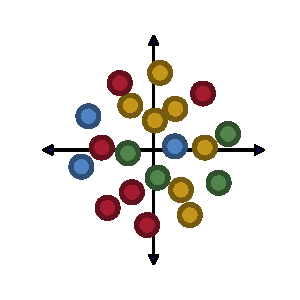
\includegraphics[width=\textwidth]{figures/ch3/new_clustered_embedded_neurons}
    \label{fig:fig1_network}
  \end{subfigure}
  \hspace{.25in}
  \begin{subfigure}[b]{1.7in}
    \centering
    \caption{}
    \vspace{-.25in}
    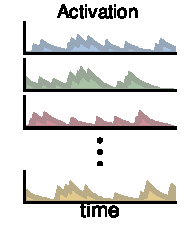
\includegraphics[width=\textwidth]{figures/ch3/new_activation}
    \label{fig:fig1_activation}
  \end{subfigure}
  \hspace{.25in}
  \begin{subfigure}[b]{1.7in}
    \centering
    \caption{}
    \vspace{-.25in}
    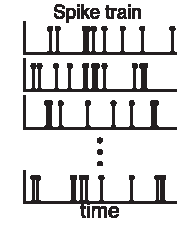
\includegraphics[width=\textwidth]{figures/ch3/new_observed_spikes}
    \label{fig:fig1_spikes}
  \end{subfigure}
  \vspace{-.2in}
  \caption[Components of the network Hawkes model]{
     Components of the generative model. 
     \textbf{(a)} Each neuron is endowed with latent variables, like 
     locations in space and discrete types (illustrated with different colors).
     These variables determine the probability of connections and the 
     strength of those connections. In this example, nearby neurons of the same 
     type are most likely to connect.
     \textbf{(b)} The network parameterizes an autoregressive model 
     with a time-varying activation, which specifies the instantaneous probability 
     of an action potential.
     \textbf{(c)} Spikes are randomly generated according to the 
     activation. Each spike induces an impulse response on the activation 
     of downstream neurons.}
  \label{fig:network_hawkes}
\end{figure}

The rest of the chapter is organized as follows. In
Section~\ref{sec:graph_models} we introduce a compositional
probabilistic model for networks, and in
Section~\ref{sec:hawkes_processes} we introduce Hawkes processes.
Section~\ref{sec:network_hawkes_model} stitches these two components
together into a joint model for implicit networks.  Before diving into
inference applications, we first consider the theoretical consequences
of a particular network model on the stability of the system, and
provide some intuition on how the network properties affect the
asymptotic behavior of the system.  Then, in
Section~\ref{sec:hawkes_inference}, we derive a Gibbs sampling
algorithm with an elegant auxiliary variable formulation.  Finally,
the remaining sections consider applications, first to synthetic data,
and then to biological recordings.  While the primary emphasis is on
modeling neural data, we also explore some applications in areas of
finance and criminology.

\section{Probabilistic Network Models}
\label{sec:graph_models}
Networks of~$N$ nodes can be represented by~${N\times N}$
matrices. Unweighted networks correspond to binary adjacency
matrices~$\bA$ where~${a_{m,n}=a_{m \to n}=1}$ indicates a directed
edge from node~$m$ to node~$n$. We use the arrow notation ($\to$) to
remind the reader of the directionality of the connection. When these
edges have scalar weights associated with them, we can encode the
weights in a second matrix,~${\bW \in \reals^{N \times N}}$.  The
complete network is then defined by the elementwise product,~${\bA
  \odot \bW}$. The binary adjacency matrix captures the sparsity
pattern, and the real-valued wieght matrix captures the strength of
the connections. From a modeling perspective, separating these two
matrices allows us to separate our prior intuitions about sparsity and
strength. This is known as a spike-and-slab model~\cite{Mitchell1988}.


Hierarchical models can be constructed by incorporating latent
variables into the prior distributions over~$\bA$ and~$\bW$.
Unsurprisingly, the same types of motifs that recur throughout
probabilistic modeling --- discrete latent types and continuous
latent features--- also form the building blocks of
standard network models.  We briefly outline a few simple models that
are used in this and following chapters.

Table~\ref{tab:A_models} summarizes a few models for binary adjacency
matrices. In all cases, the distribution over~$\bA$ factorizes into a
product over edges,
\begin{align*}
  p(\bA \given \bz, \bvartheta)
  &= \prod_{n=1}^N \prod_{n'=1}^N p(a_{n \to n'} \given \bz_n, \bz_{n'}, \bvartheta) \\
  &= \prod_{n=1}^N \prod_{n'=1}^N \distBernoulli(a_{n \to n'} \given \rho_{n \to n'}).
\end{align*}
The difference is in how the local latent variables,~$\bz_{n'}$
and~$\bz_n$, and the global network parameters,~$\bvartheta$, combine to
determine the probability,~$\rho_{n \to n'}$. We describe these models
below:
\begin{itemize}
\item \textit{Empty Model: } The empty model is essentially a null
  model. According to this model, there are no connections between
  neurons. Nevertheless, it is useful to enumerate it here because
  the empty model provides a baseline for more sophisticated models
  by capturing the null hypothesis that neurons are independent. 
  
\item \textit{Dense Model: } On the other extreme, the dense model
  corresponds to the hypothesis that all pairs of neurons are
  connected. In the models of neural activity that follow, the
  dense model will reduce to the standard models in use today, which
  do not incorporate prior distributions over the network.
  
\item \textit{Bernoulli Model: } The Bernoulli model is a
  spike-and-slab model in which each connection is an independent and
  identically distributed Bernoulli random variable with
  probability~$\rho$. This is also known as an Erd\"os-R\'enyi model.
  
\item \textit{Stochastic Block Model (SBM): } In the stochastic block
  model (SBM) \cite{Nowicki-2001}, each neuron has an associated
  class,~$z_n$.  The probability of connection depends on the class of
  the two neurons.  This is the network equivalent of a mixture model.
  In a Bayesian framework, we assume the class assignments are drawn
  from a categorical prior,~${z_n \sim \distCategorical(\bpi)}$, and
  the class weights are given a conjugate, symmetric Dirichlet
  prior,~${\bpi \sim \distDirichlet(\alpha \bone_K)}$. The connection
  probabilities are given a conjugate beta prior,~${\beta_{k \to k'}
    \sim \distBeta(\alpha, \beta)}$.
  
\item \textit{Latent Distance Model: } The latent distance model
  \cite{Hoff-2008} encodes the belief that connection probability
  should decrease with distance between latent locations. The
  locations are given spherical Gaussian priors,~$\bz_n \sim
  \distNormal(0, \tau \bI)$, and the scale is drawn from an inverse
  gamma prior,~$\tau \sim \distInvGamma(1,1)$. The offset is given a
  standard normal prior,~$\gamma_0 \sim \distNormal(0, 1)$.

\end{itemize}
\begin{table}
\begin{center}
\begin{tabular}{c|c|c|c}
Name & $\bvartheta$ & $\mathrm{dom}(\bz_n)$ & $\rho_{n \to n'}$ \\
\hline
Empty Model & --- &  --- & $0$ \\
Dense Model & --- & --- & $1$ \\
Bernoulli Model & $\rho$ & --- & $\rho$ \\
Stochastic Block Model & $\{\{\rho_{k \to k'}\}\}$ & $\{1, \ldots, K\}$ & $\rho_{z_n \to z_{n'}}$ \\
Latent Distance Model & $\gamma_0$ & $\reals^K$ & $\sigma(-||\bz_n - \bz_{n'}||_2^2 + \gamma_0)$
\end{tabular}
\end{center}
\caption{Binary adjacency matrix models.}
\label{tab:A_models}
\end{table}



% Weight models
\begin{table}
\begin{center}
\begin{tabular}{c|c|c|c}
Name & $\bvartheta$ & $\mathrm{dom}(\bz)$ & $\mu_{n \to n'}$ \\
\hline
Independent Model & $\mu$ & --- & $\mu$ \\
Stochastic Block Model & $\{\{ \mu_{k \to k'} \}\}$ & $\{1, \ldots, K\}$ & $\mu_{z_n \to z_{n'}}$ \\
Latent Distance Model & $\mu_0$ & $\reals^K$ & $-||\bz_n - \bz_{n'}||_2^2 + \mu_0$ 
\end{tabular}
\end{center}
\caption{General weight models.}
\label{tab:W_models}
\end{table}

The same ideas can be applied to models for the scalar weight matrix,~$\bW$,
but rather than modeling the connection probability, we now model the
mean weight,~$\mu_{n \to n'}$. The resulting distribution is of the form,
\begin{align*}
  p(\bW \given \bz, \bvartheta)
  &= \prod_{m=1}^N \prod_{n=1}^N p(w_{m \to n} \given z_n, z_{n'}, \bvartheta) \\
  &= \prod_{m=1}^N \prod_{n=1}^N p(w_{m \to n} \given \mu_{m \to n}, \bvartheta).
\end{align*}

We do not specify the exact functional form of the distribution since
this will depend on the model for neural activity. The linear
models with non-negative weights in this chapter will use a gamma
prior, whereas the nonlinear autoregressive models in Chapter~\ref{chap:five} will use a Gaussian
distribution. Table~\ref{tab:W_models} lists some examples of weight
models analogous to the adjacency matrix models above.
While we have only shown models for the mean weight,
the same latent variables may
also parameterize the variance of the weight distribution. For example
in a Gaussian SBM, each directed pair of classes may have an
associated variance,~$\sigma^2_{k \to k'}$.

Probabilistic network models like these are unified under an elegant
theoretical framework due to Aldous and Hoover
\cite{Aldous-1981,Hoover-1979}. Conceptually, the Aldous-Hoover
representation characterizes the class of \textit{exchangeable} random
graphs, that is, graph models for which the joint probability is
invariant under permutations of the node labels. Just as de Finetti's
theorem equates exchangeable sequences to independent draws from a
random probability measure, Aldous-Hoover renders the entries of~$\bA$ and~$\bW$ conditionally
independent given latent variables~$\bz$ and global
parameters~$\bvartheta$. \citet{Lloyd-2012} and~\citet{orbanz2015bayesian}
review this theoretical framework and its applications in
probabilistic machine learning.

% Network models
\begin{figure}[t!]
  \centering
  \textit{~~~~~Adjacency Model} \\
  % Gaussian row
  \hspace{1em}
  \begin{subfigure}[b]{1.25in}
    \centering
    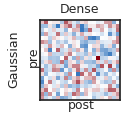
\includegraphics[width=\textwidth]{figures/ch3/Dense-Gaussian.png}
  \end{subfigure}
  ~
  \hspace{-.1in}
  \begin{subfigure}[b]{1.10in}
    \centering
    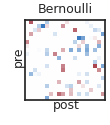
\includegraphics[width=\textwidth]{figures/ch3/Bernoulli-Gaussian.png}
  \end{subfigure}
  ~
  \hspace{-.1in}
  \begin{subfigure}[b]{1.10in}
    \centering
    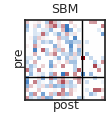
\includegraphics[width=\textwidth]{figures/ch3/SBM-Gaussian.png}
  \end{subfigure}
  ~
  \hspace{-.1in}
  \begin{subfigure}[b]{1.10in}
    \centering
    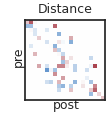
\includegraphics[width=\textwidth]{figures/ch3/Distance-Gaussian.png}
  \end{subfigure}
  \\
  \vspace{-.1in}
  % SBM row
  \rotatebox{90}{\textit{~~~~~Weight Model}}
  \begin{subfigure}[b]{1.25in}
    \centering
    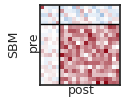
\includegraphics[width=\textwidth]{figures/ch3/Dense-SBM.png}
  \end{subfigure}
  ~
  \hspace{-.1in}
  \begin{subfigure}[b]{1.10in}
    \centering
    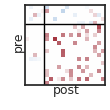
\includegraphics[width=\textwidth]{figures/ch3/Bernoulli-SBM.png}
  \end{subfigure}
  ~
  \hspace{-.1in}
  \begin{subfigure}[b]{1.10in}
    \centering
    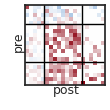
\includegraphics[width=\textwidth]{figures/ch3/SBM-SBM.png}
  \end{subfigure}
  ~
  \hspace{-.1in}
  \begin{subfigure}[b]{1.10in}
    \centering
    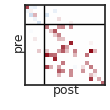
\includegraphics[width=\textwidth]{figures/ch3/Distance-SBM.png}
  \end{subfigure}
  \\
  % Distance row
  \vspace{-.1in}
  \hspace{1em}
  \begin{subfigure}[b]{1.25in}
    \centering
    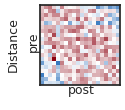
\includegraphics[width=\textwidth]{figures/ch3/Dense-Distance.png}
  \end{subfigure}
  ~
  \hspace{-.1in}
  \begin{subfigure}[b]{1.10in}
    \centering
    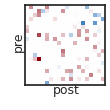
\includegraphics[width=\textwidth]{figures/ch3/Bernoulli-Distance.png}
  \end{subfigure}
  ~
  \hspace{-.1in}
  \begin{subfigure}[b]{1.10in}
    \centering
    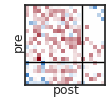
\includegraphics[width=\textwidth]{figures/ch3/SBM-Distance.png}
  \end{subfigure}
  ~
  \hspace{-.1in}
  \begin{subfigure}[b]{1.10in}
    \centering
    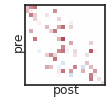
\includegraphics[width=\textwidth]{figures/ch3/Distance-Distance.png}
  \end{subfigure}
  \\
  \vspace{-.1in}
  \caption[Examples of network models]{Example network models.  Each
    row corresponds to a fixed weight matrix,~$\bW$, for three
    different weight models, and each column corresponds to a fixed
    adjacency matrix,~$\bA$, for four different adjacency models. The
    panels show the elementwise product of the two. Color denotes the
    weight (blue is negative, red is postiive).  In the SBM, the rows
    and columns are sorted by type, and in the distance model, they
    are sorted by location. }
  \label{fig:network_models}
\end{figure}

Note that we have associated each neuron with a single latent variable,~$\bz_n$.
This suggests that both the adjacency matrix and the weight matrix are
governed by the same latent variable, but in general they can have separate
variables. Whether or not they are shared is a modeling decision. We will
collectively refer to all latent variables of the network as~$\bz_n$ and
whether they govern the adjacency model or the weight model will be clear
from context.


Figure~\ref{fig:network_models} shows how a variety of networks can be
constructed by combining different priors on the weights (rows) with
priors on the pattern of connectivity (columns). Each row corresponds
to a fixed weight matrix drawn from either an independent model, a
stochastic block model (SBM), or a latent distance model. In these
cases, the weights are Gaussian distributed with unit variance and
model-specific mean. Each column corresponds to a fixed adjacency
matrix drawn from either a dense model, an independent
Bernoulli model, an SBM, or a latent distance model. The matrices show
the element-wise product, which encodes a weighted, directed
network. Next, we introduce a model for spike trains that leverages
an underlying network.


\section{Hawkes Processes}
\label{sec:hawkes_processes}
Hawkes processes \cite{Hawkes-1971} are a special type of point process
that allow spikes to influence the future firing rate. This is achieved
via a linear superposition of Poisson processes. Before jumping into the
details, a brief primer on Poisson processes is in order.

\subsection{Poisson Processes}
\sloppy Point processes are fundamental statistical objects that yield
random finite sets of spikes~${\{s_m\}_{m=1}^M \subset \mcV}$,
where~$\mcV$ is a compact subset of~${\reals^D}$.  When modeling
neural spike trains, we typically let~${\mcV}$ be the
interval~${[0,T]}$. The Poisson process is the canonical example. It
is governed by a nonnegative firing rate or intensity
function,~${\lambda(t): \mcV \rightarrow\reals_+}$. The number of
spikes in a subset~${\mcV'\subset\mcV}$ follows a Poisson distribution
with mean~${\int_{\mcV'}\lambda(t) \, \mathrm{d}t}$. Moreover, the number
of spikes in disjoint subsets are independent.

We use the notation~${\{s_m\}_{m=1}^M\sim\PP(\lambda(t))}$ to indicate
that a set of spikes~$\{s_m\}_{m=1}^M$ is drawn from a Poisson process
with rate~$\lambda(t)$. There are many ways to sample a Poisson
process; one way is to sample a Poisson number of spikes with
mean~${\int_{\mcV} \lambda(t) \mathrm{d}t}$ and then sample the individual
spike times,~$s_m$, independently from the density,
%\begin{align*}
${
  p(s) = \frac{\lambda(s)}{\int_{\mcV} \lambda(t) \, \mathrm{d}t}.
}$
%\end{align*}
Thus, after accounting for the~$M!$ permutations,
the likelihood of a set of spikes is given by,
\begin{align}
  \nonumber
  p(\{s_m\}_{m=1}^M \given \lambda(t))
  &= \distPoisson \left(M \, \bigg| \, \int_{\mcV} \lambda(t) \, \mathrm{d} t \right)
  \left( \prod_{m=1}^M \frac{\lambda(s_m)}{\int_{\mcV} \lambda(t) \, \mathrm{d}t} \right)  M! \\
  \nonumber
  &= \frac{M!}{M!} \left(\int_{\mcV} \lambda(t) \, \mathrm{d} t \right)^M
  \exp \left \{-\int_{\mcV} \lambda(t) \, \mathrm{d} t \right \} 
  \left( \prod_{m=1}^M \frac{\lambda(s_m)}{\int_{\mcV} \lambda(t) \, \mathrm{d}t} \right) \\
  \label{eq:poisson_lkhd}
  &=\exp\left\{-\int_{\mathcal{V}}\lambda(t)\mathrm{d}t \right\}
  \prod_{m=1}^M\lambda(s_m).
\end{align}

\paragraph{Poisson Superposition Principle}
We will make use of a special property of Poisson processes called the
\emph{Poisson superposition principle}, which states that if we have 
sets of spikes from independent Poisson processes, then the union of spikes 
is distributed according to a Poisson process as well.
Moreover, the rate of this process equals the sum of 
rates from the individual processes. 
Formally, suppose we are given sets of spikes drawn independently
from ~$K$ Poisson processes with rates~${\lambda_1(t), \ldots,
  \lambda_K(t)}$.  Call the union of the spikes~${\{s_m,
  \omega_m\}}$, where~${s_m \in \mcV}$ is the location of the spike
and~${\omega_m \in \{1, \ldots, K\}}$ says which process it came
from. Let~${\lambda_{\mathsf{tot}}(t) = \sum_{k=1}^K \lambda_k(t)}$.
The likelihood of the full set of spikes is,
\begin{align*}
  p(\{s_m, \omega_m\}_{m=1}^M \given \{\lambda_k(t)\}_{k=1}^K)
  &= \prod_{k=1}^K \PP(\{s_m: \omega_m=k\} \given \lambda_k(t)) \\
  &= \prod_{k=1}^K \left[
    \exp\left\{-\int_{\mcV} \lambda_k(t) \, \mathrm{d}t\right\}
    \prod_{m=1}^M \lambda_k(s_m)^{\bbI[\omega_m = k]} \right] \\
  &= \exp\left\{-\int_{\mcV} \lambda_{\mathsf{tot}}(t) \, \mathrm{d}t\right\}
  \prod_{m=1}^M \prod_{k=1}^K \lambda_k(s_m)^{\bbI[\omega_m = k]}.
\end{align*}

The Poisson superposition principle says that the marginal distribution
summing over all possible process assignments,~$\{\omega_m\}$, is a Poisson
process with rate~$\lambda_{\mathsf{tot}}(t)$. To show this, we sum over
the process assignments to get,
\begin{align*}
  p(\{s_m\}_{m=1}^M \given \{\lambda_k(t)\}_{k=1}^K)
  &= \sum_{\omega_1=1}^K \cdots \sum_{\omega_M=1}^K p(\{s_m, \omega_m\}_{m=1}^M \given \{\lambda_k(t)\}_{k=1}^K) \\
  &= \exp\left\{-\int_{\mcV} \lambda_{\mathsf{tot}}(t) \, \mathrm{d}t\right\}
  \prod_{m=1}^M \sum_{\omega_m=1}^K \prod_{k=1}^K \lambda_k(s_m)^{\bbI[\omega_m = k]} \\
  &= \exp\left\{-\int_{\mcV} \lambda_{\mathsf{tot}}(t) \, \mathrm{d}t\right\}
  \prod_{m=1}^M \lambda_{\mathsf{tot}}(s_m) \\
  &= \PP(\{s_m\} \given \lambda_{\mathsf{tot}}(t)).
\end{align*}
Furthermore, the conditional distribution of~$\omega_m$ is,
\begin{align*}
  p(\omega_m=k \given s_m, \{\lambda_k(t)\}_{k=1}^K)
  &= \frac{\lambda_k(s_m)}{\sum_{k'=1}^K \lambda_{k'}(s_m)}.
\end{align*}
In other words, given a set of spikes drawn from rate~$\lambda_{\mathsf{tot}}(t)$,
we can attribute each spike to one of the~$K$ additive contributions
to the rate function by sampling a categorical distribution with probabilities
given by the relative rate at the time of the spike. This is known as
\emph{Poisson thinning}.

\subsection{Including Spike History with Hawkes Processes}
Though Poisson processes have many nice properties, they cannot
capture interactions between spikes. For this we turn to a more
general model known as Hawkes processes \cite{Hawkes-1971}. 
First, consider the spike train of a single neuron,~$\{s_m\}_{m=1}^M \subset [0,T]$.
In a Hawkes process, the firing rate at time,~$\lambda(t \given \mcH_t)$, is a function of 
the spike history,~${\mcH_t = \{s_m: s_m < t\}}$.  The neuron has a 
baseline firing rate,~$\lambda^{(0)}$. On top of this baseline, 
each spike 
adds a nonnegative impulse response,~$h(\Delta t)$, to the 
subsequent firing rate.  This allows for spike-driven dynamics that are not possible in Poisson
processes.  Causality and
locality of influence are enforced by limiting the support of~$h(\Delta
t)$ to~${\Delta t \in [0,\Delta t_{\mathsf{max}}]}$.
The rate is thus given by,
\begin{align*}
  \lambda(t \given \mcH_t)
  &= \lambda^{(0)} + \sum_{m=1}^M h(t - s_m).
\end{align*}
When the impulse response is equal to zero, the Hawkes process
reduces to a standard Poisson process with rate~$\lambda^{(0)}$.

By the superposition theorem for Poisson processes, these additive
components can be considered independent processes, each giving rise
to their own spikes.  This suggests a convenient latent variable
representation in which each spike is attributed to either the
background rate or the impulse response of a preceding spike.  We
augment our data with a latent random
variable~${\omega_m \in\{0,\ldots, m-1\}}$ to indicate the \emph{origin} of
the~$m$-th spike ($0$ if the spike is due to the background rate and
${1\ldots m-1}$ if it was spawned by a preceding spike). 

This is easily extended to a population of~$N$ neurons by considering a Hawkes
process that gives rise to sets of
\emph{marked} spikes $\{s_m,c_m\}_{m=1}^M$,
where~${c_m\in\{1,\ldots,N\}}$ specifies the neuron on which
the~$m$-th spike occurred.  As in the single neuron case, 
the rate of the~$n$-th neuron,~${\lambda_n(t\given
  \mcH_t)}$,  depends on the spike history, but here the spike history 
contains the spikes of all neurons through time~$t$. 
The multineuronal generalization also allows for different background rates 
for each neuron,~$\lambda^{(0)}_{n}$, and  different impulse 
responses for each pair of neurons. For example, the impulse 
response from neuron~$n$ to neuron~$n'$, which we now call~$h_{n \to n'}$, 
may differ from that of the reverse connection. As before, we
do require that the impulse responses be causal and have bounded support.
Putting it all together, the rate of the~$n$-th neuron is,
\begin{align}
  \label{eq:hawkes_rate}
  \lambda_n(t \given \mcH_t)
  &= \lambda^{(0)}_{n}(t) + \sum_{m=1}^M h_{c_m \to n}(t - s_m).
\end{align}

\begin{figure}[t]
\centering%
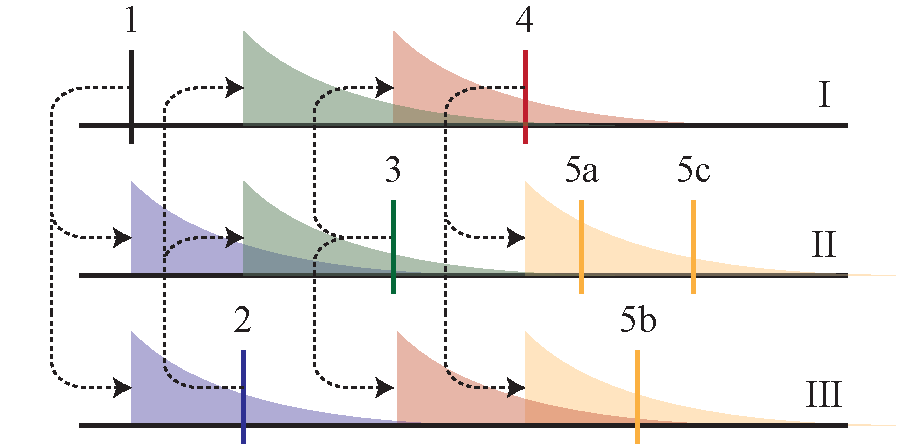
\includegraphics[width=4in]{figures/ch2/Hawkes-wide} 
\vspace{-0.25cm}
\caption[Illustration of a Hawkes process]{Illustration of a Hawkes
  process. Spikes induce impulse responses on connected processes and
  spawn ``child'' spikes. See the main text for a complete
  description.}
\label{fig:hawkes}
\end{figure}

After augmenting the data with auxiliary variables denoting the origin
of each spike, the multineuronal Hawkes process likelihood reduces to 
a product of Poisson process likelihoods for each background rate and 
each impulse response:
\begin{multline*}
  p(\{(s_m,c_m,\omega_m)\}_{m=1}^M \given 
  \{\lambda^{(0)}_{n}(t)\}, \{\{h_{n \to n'}(\Delta t)\}\}) = \\
  \prod_{n=1}^N \PP \big(\{s_{m}: c_{m}=n \wedge \omega_{m}=0\} \given \lambda^{(0)}_{n}(t) \big) \; \times\\
  \prod_{m=1}^M \prod_{n'=1}^N \PP \big(\{s_{m'}: c_{m'}=n' \wedge \omega_{m'}=m\} \given h_{c_m \to n'}(t-s_m) \big).
\end{multline*}
Combining this with 
Eq.~\ref{eq:poisson_lkhd}, we can
write the augmented likelihood as,
\begin{multline}
  \label{eq:hawkes_likelihood}
  p(\{s_m, c_m, \omega_m\}_{m=1}^M \given \{\lambda^{(0)}_{n}\}, \{\{h_{n \to n'}(\Delta t)\}\}) = \\
  \prod^N_{n=1} \bigg[
  \exp\left\{ -\int_0^T \lambda^{(0)}_{n}(t)\mathrm{d}t \right\} \,
  \prod^M_{m=1}
   \lambda^{(0)}_{n}(s_m)^{\bbI[c_m=n] \bbI[\omega_m = 0]} \bigg]\\
  \quad\times \prod_{m=1}^M \prod_{n'=1}^N \bigg[
  \exp\left\{-\int^T_{s_m} h_{c_m \to n'}(t - s_m) \mathrm{d}t \right\} \\
  \prod_{m'=1}^M h_{c_m^{~} \to c_{m'}}(s_{m'}-s_m)^{\bbI[c_{m'}=n'] \bbI[\omega_{m'}=m]}\bigg].
\end{multline}
The second line corresponds to the likelihood of the background
processes; the third and fourth correspond to the likelihood of the
induced processes triggered by each spike.

Figure~\ref{fig:hawkes} illustrates a causal cascades of spikes for a
simple network of three processes (I-III).  The first spike is caused
by the background rate~(${\omega_1=0}$), and it induces impulse responses
on processes II and III. Spike~2 is spawned by the impulse on the
third process~(${\omega_2=1}$), and feeds back onto processes I and II. In
some cases a single parent spike induces multiple children, e.g.,
spike~4 spawns spikes~{5a-c}. In this simple example, processes excite
one another, but do not excite themselves.

\section{The Network Hawkes Model}
\label{sec:network_hawkes_model}
In order to combine Hawkes processes and random network models, we
decompose the Hawkes impulse response $h_{n \to n'}(\Delta t)$ as
follows:
\begin{align}
\label{eq:ir_decomp}
h_{n \to n'}(\Delta t) &= a_{n \to n'} \cdot w_{n \to n'} \cdot \hbar(\Delta t; \theta_{n \to n'}).
\end{align}
Here,~$a_{n \to n'}$ is an entry in the binary adjacency
matrix,~${\bA\in\{0,1\}^{N \times N}}$,
and~$w_{n \to n'}$ is the corresponding entry in the non-negative
weight matrix,~${\bW \in\reals_+^{N\times N}}$. Together these specify
the \emph{sparsity structure} and \emph{strength} of the interaction
network, respectively. The non-negative function~${\hbar(\Delta t;
  \theta_{n \to n'})}$ captures the temporal aspect of the
interaction. It is parameterized by~${\theta_{n \to n'}}$ and
satisfies two properties: a) it has bounded support for~${\Delta t \in
  [0,\Delta t_{\mathsf{max}}]}$, and~b) it integrates to one. In other
words,~$\hbar$ is a probability density with compact support.

Decomposing the impulse response as in Equation~\ref{eq:ir_decomp} has
many advantages. It allows us to express our separate beliefs about
the sparsity structure of the interaction network and the strength of
the interactions by using probabilistic network models as priors
on~$\bA$ and~$\bW$.  The empty graph model recovers independent
background processes, and the complete graph recovers the standard
Hawkes process introduced by \citet{Hawkes-1971}.  Making~$\hbar$ a
probability density endows~$\bW$ with units of ``expected number of
spikes'' and allows us to compare the relative strength of
interactions. The form suggests an intuitive generative model: for
each impulse response draw~${k \sim \text{Poisson}(w_{n \to n'})}$
number of induced spikes and draw the~$k$ child spike times
i.i.d.\ from~$\hbar$.  
As we will see, this enables computationally
tractable conjugate priors.

We can now write down the joint probability of the probabilistic model,
\begin{multline}
\label{eq:hawkes_complete_model}
p(\{s_m, c_m, \omega_m\}, \bA, \bW, \{\{\theta_{n \to n'}\}\}, \{\lambda^{(0)}_{n}\}, \{\bz_n\}, \bvartheta \given \boldeta) 
=  \\
p(\bvartheta \given \boldeta)
\times \overbrace{p(\{\bz_n\} \given \bvartheta, \boldeta)}^\text{latent variables}
\times \overbrace{p(\bA, \bW \given \{\bz_{n}\}, \bvartheta, \boldeta)}^\text{network} 
\times \overbrace{p(\{\lambda^{(0)}_{n}\} \given \boldeta)}^\text{background}
\times \overbrace{p(\{\theta_{n\to n'}\} \given \boldeta)}^\text{impulses} \\
\times \overbrace{  p \left(\{s_m, c_m, \omega_m\} \given \bA, \bW, \{\theta_{n \to n'}\}, \{\lambda^{(0)}_{n}\} \right) }^\text{augmented likelihood}.
\end{multline}
Before deriving inference algorithms for this model, however, we pause 
to consider some of its theoretical properties.


% Intuitively, the background rates,~$\lambda^{(0)}_{n}(t)$, explain spikes
% that cannot be attributed to preceding spikes. In the simplest case
% the background rate is constant. However, there are often fluctuations
% in overall intensity that are shared among the processes, and not
% reflective of process-to-process interaction, as we will see in the
% daily variations in trading volume on the S\&P100 and the seasonal
% trends in homicide. To capture these shared background fluctuations,
% we use a sparse log Gaussian Cox process \cite{Moller-1998} to model
% the background rate:
% \begin{align*}
%   \lambda^{(0)}_{n}(t)
%   & = \mu_{n} + \alpha_{n}\exp\{\by(t)\}, \\
%   \by(t) &\sim \mathcal{GP}(\boldsymbol{0},K(t,t')).
% \end{align*}

% The kernel~${K(t,t')}$ describes the covariance structure of the
% background rate that is shared by all processes. For example, a
% periodic kernel may capture seasonal or daily fluctuations. The
% offset~${\mu_n}$ accounts for varying background intensities among
% processes, and the scaling factor~$\alpha_n$ governs how sensitive
% process~$n$ is to these background fluctuations (when~${\alpha_n=0}$
% we recover the constant background rate).

% Finally, in some cases the process identities,~${c_m}$, must also be
% inferred. With gang incidents in Chicago we may have only a
% location,~${\bx_m\in\reals^2}$. In this case, we may place a spatial
% Gaussian mixture model over the~$c_m$'s, as in
% \citet{Cho-2013}. Alternatively, we may be given the label of the
% community in which the incident occurred, but we suspect that
% interactions occur between clusters of communities. In this case we
% can use a simple clustering model or a nonparametric model like that
% of \citet{Blundell-2012}.

\subsection{Stability of Network Hawkes Processes}
\label{sec:stability}


Due to their recurrent, mutually-exciting nature, Hawkes processes
an unconstrained system can easily be unstable and lead to an infinite 
number of spikes. A stable system must satisfy \footnote{In
  this context,~${\lambda_{\mathsf{max}}}$ refers to an eigenvalue
  rather than a rate.}
\begin{align*}
  \lambda_{\mathsf{max}}=\max\; |\,\mathrm{eig}(\bA\odot\bW)\,| < 1
\end{align*}
(c.f. \citet{Daley-1988}).
For the generative model, we would like
to set our hyperparameters such that the prior distribution places
little mass on unstable networks. In order to do so, we use tools from
random matrix theory.

The circular law describes the asymptotic eigenvalue distribution for
$N \times N$~random matrices with entries that are i.i.d. with zero
mean and variance~$\sigma^2$. As~$N$ grows, the eigenvalues are
uniformly distributed over a disk in the complex plane centered at the
origin and with radius~$\sigma\sqrt{N}$. In our case, however, the
mean of the entries,~${\mu=\mathbb{E}[a_{n \to n'} \cdot w_{n \to
      n'}]}$, is not zero. \citet{Silverstein-1994} has analyzed such
``noncentral'' random matrices and shown that the largest eigenvalue
is asymptotically distributed
as~${\lambda_{\sf{max}} \sim \distNormal(\mu N,\, \sigma^2)}$.

In the simple case of~${w_{n \to n'}\sim \distGamma(\kappa,\nu)}$
and~${a_{n \to n'}\sim\distBernoulli(\rho)}$, we have
${\mu = \rho \kappa/\nu}$ and
${\sigma=\sqrt{\rho((1-\rho)\kappa^2+\kappa)}/\nu}$. We are using the 
rate parameterization of the gamma distribution, 
\begin{align*}
\distGamma(w \given \kappa, \nu) &= \frac{\nu^{\kappa}}{\Gamma(\kappa)}w^{\kappa- 1} e^{-\nu w}.
\end{align*}
For a
given~$N$,~$\kappa$ and~$\nu$, we can tune the sparsity
parameter~$\rho$ to achieve stability with high probability. We simply
set~$\rho$ such that the minimum of~$\sigma\sqrt{N}$ and,
say,~${\mu N + 3\sigma}$, equals one. Figures~\ref{fig:stability_p_w}
and~\ref{fig:stability_max_rho} show a variety of weight distributions
and the maximum stable~$\rho$. Increasing the network size, the mean,
or the variance will require a concomitant increase in sparsity.

\begin{figure}[t]
\vspace{-.5em}
\begin{center}
\begin{subfigure}[b]{.22\textwidth}
\caption{}
\label{fig:stability_p_w}
%\vspace{-.9em}
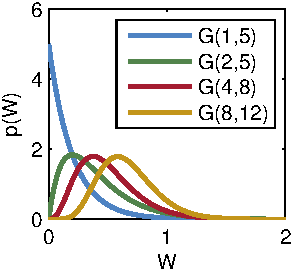
\includegraphics[height=1.25in]{figures/ch2/stability_p_w} 
\end{subfigure}
~
\begin{subfigure}[b]{.22\textwidth}
\caption{}
%\vspace{-1em}
\label{fig:stability_max_rho}
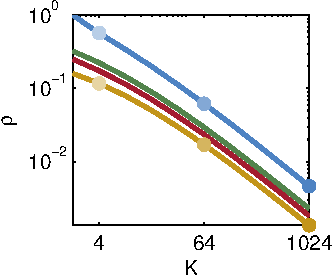
\includegraphics[height=1.25in]{figures/ch2/stability_max_rho} 
\end{subfigure}
~
\hspace{1em}
\begin{subfigure}[b]{.22\textwidth}
\caption{}
\label{fig:stability_1_5}
%\vspace{-.5em}
%\vspace{.8em}
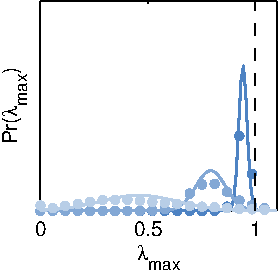
\includegraphics[height=1.2in]{figures/ch2/stability_1_5} 
\end{subfigure}
~
\begin{subfigure}[b]{.22\textwidth}
%\vspace{.7em}
\caption{}
\label{fig:stability_8_12}
%\vspace{-.5em}
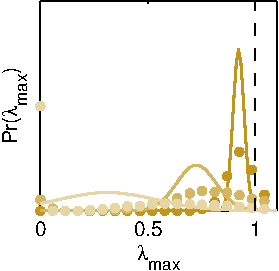
\includegraphics[height=1.2in]{figures/ch2/stability_8_12} 
\end{subfigure}
\end{center}
\vspace{-1em}
\caption[Distribution of the maximum eigenvalue for Erd\H{o}s-Renyi
  graphs with gamma weights]{Empirical and theoretical distribution of
  the maximum eigenvalue for Erd\H{o}s-Renyi graphs with gamma
  weights. (a) Four gamma weight distributions. The colors correspond
  to the curves in the remaining panels. (b) Sparsity that
  theoretically yields ${99\%}$ probability of stability as a function
  of~${p(w)}$ and~$N$. (c) and (d) Theoretical (solid) and empirical
  (dots) distribution of the maximum eigenvalue. Color corresponds to
  the weight distribution in (a) and intensity indicates~$N$
  and~$\rho$ shown in (b).}
\label{fig:stability}
\end{figure}

 
This approach relies on asymptotic eigenvalue distributions, and it is
unclear how quickly the spectra of random matrices will converge to
this distribution. To test this, we computed the empirical eigenvalue
distribution for random matrices of various size, mean, and
variance. We generated~$10^4$ random matrices for each weight
distribution in Figure~\ref{fig:stability_p_w} with sizes~$N=4$,~$64$,
and~$1024$, and~$\rho$ set to the theoretical maximum indicated by
dots in Figure~\ref{fig:stability_max_rho}. The theoretical and
empirical distributions of the maximum eigenvalue are shown in
Figures~\ref{fig:stability_1_5} and~\ref{fig:stability_8_12}. We find
that for small mean and variance weights, for
example~$\distGamma(1,5)$ in the Figure~\ref{fig:stability_1_5}, the
empirical results closely match the theory. As the weights grow
larger, as in~${\distGamma(8,12)}$ in~\ref{fig:stability_8_12}, the
empirical eigenvalue distributions have increased variance and lead to
a greater than expected probability of unstable matrices for the range
of network sizes tested here. We conclude that networks with strong
weights should be counterbalanced by strong sparsity limits, or
additional structure in the adjacency matrix that prohibits excitatory
feedback loops.


\section{Bayesian Inference with Gibbs Sampling}
\label{sec:hawkes_inference}
We present a Gibbs sampling procedure for inferring the model
parameters,~$\bA$,~$\bW$, $\{\lambda^{(0)}_{n}\}$, $\{\theta_{n \to n'}\}$,
and the paremeters of the network,~$\{\bz_n\}$ and~$\bvartheta$.
In order to simplify our Gibbs updates, we
will also sample a set of parent assignments for each
spike~$\{\omega_m\}$. Incorporating these parent variables enables
conjugate prior distributions and simple and efficient Gibbs sampling
algorithm.

\paragraph{Sampling weights $\bW$.} 
To derive the updates for weights, recall from
Equation~\ref{eq:ir_decomp} that~${w_{n \to n'}}$ only
appears in the impulse responses for which~${c_m=n}$
and~${c_{m'}=n'}$, so the likelihood is propotional to,
\begin{align*}
  p(\{s_m, c_m, & \omega_m\}^M_{m=1} \given a_{n \to n'}, w_{n \to n'}, 
  \theta_{n \to n'}) \\
  &\propto \prod_{m=1}^M\left[
    \exp\left\{-\int^T_{s_m} a_{n \to n'} \cdot w_{n \to n'} \cdot \hbar(t - s_m; \theta_{n \to n'}) \, \mathrm{d}t
    \right\} \right]^{\bbI[c_m=n]} \\
  &\qquad \times \prod_{m=1}^M \prod_{m'=1}^M \bigg[
    w_{n \to n'}\bigg]^{\bbI[c_{m}=n] \bbI[c_{m'}=n'] \bbI[\omega_{m'}=m]}.
\end{align*}
If~${a_{n \to n'}=0}$, the impulse response is deterministically zero
and, as a result, none of the spikes on neuron~$n'$ will be attributed to spikes
on neuron~$n$. Thus, the likelihood reduces to the prior,~$p(w_{n \to n'})$.
If~${a_{n \to n'}=1}$, the likelihood is more complicated.
Note, however, that if~$s_m < T - \Delta t_{\mathsf{max}}$,
\begin{align*}
  -\int^T_{s_m} a_{n \to n'} \cdot w_{n \to n'} \cdot
  \hbar(t - s_m; \theta_{n \to n'}) \, \mathrm{d}t
  &= -w_{n \to n'}  \int^T_{s_m} \hbar(t - s_m; \theta_{n \to n'}) \, \mathrm{d}t \\
  &= - w_{n \to n'},
\end{align*}
since~$\hbar$ is a density defined on~$[0,\Delta t_{\mathsf{max}}]$.
In general, it is safe to ignore the impulse responses from spikes that 
occur in the time after~$T-\Delta t_{\mathsf{max}}$ since this will be 
quite small compared to the total recording. 
With this approximation, the conditional distribution of~$w_{n \to n'}$
reduces to,
\begin{align*}
  p(\{s_m,c_m, \omega_m\}^M_{m=1} \given a_{n \to n'}=1, w_{n \to n'}) 
  \propto 
  e^{-M_n \cdot w_{n \to n'}}  \,
  (w_{n \to n'})^{M_{n \to n'}}.
\end{align*}
where
\begin{align*}
  M_{n} &= \sum_{m=1}^M \bbI[c_{m}=n], \\
  M_{n \to n'} &= \sum_{m=1}^M \bbI[c_{m}=n] \, \bbI[c_{m'}=n'] \, \bbI[\omega_{m'}=m].
\end{align*}
These sufficient statistics count the number of spikes caused
by an connection~${n \to n'}$ and the total unweighted rate induced by
spikes on neuron~$n$.

Now that we have simplified the augmented log likelihood, we see that
it is conjugate with a gamma prior on the weights, ${w_{n \to n'} \sim
  \distGamma(\kappa_{n \to n'}, \nu_{n \to n'}})$.  In
Section~\ref{sec:graph_models} the weight models specified the
mean,~$\mu_{n \to n'}$.  For a gamma distribution,~${\mu_{n \to n'} =
  \frac{\kappa_{n \to n'}}{\nu_{n \to n'}}}$. The simplest way to
reconcile these is to fix the shape parameter~${\kappa_{n \to n'}
  \equiv \kappa}$, then we can compute the rate,~$\nu_{n \to n'}$
for any given mean. 

Assuming~$\kappa$ and~$\nu_{n \to n'}$ are given,
the conditional distribution of the weights is,
\begin{align*}
  p(w_{n \to n'}\given \{s_m,c_m,\omega_m\}_{m=1}^M, a_{n\to n'}=1, \kappa, \nu_{n \to n'})
  &= 
  \distGamma(w_{n \to n'} \given \widetilde{\kappa}_{n \to n'}, \widetilde{\nu}_{n \to n'}),
\end{align*}
where
\begin{align*}
  \widetilde{\kappa}_{n \to n'} &= \kappa + M_{n \to n'}, \\
  \widetilde{\nu}_{n \to n'} &= \nu_{n \to n'} + M_n.
\end{align*}


\paragraph{Sampling constant background rates.}
Similarly, the likelihood of a constant background rate,
${\lambda^{(0)}_{n}}$, is conjugate with a gamma
prior~${\lambda^{(0)}_{n} \sim
  \distGamma(\alpha_{\lambda},\beta_{\lambda})}$.  The conditional
distribution is,
\begin{align*}
  p(\lambda^{(0)}_{n} \given \{s_m,c_m, \omega_m\}_{m=1}^M, \alpha_\lambda, \beta_\lambda)
  &=
  \distGamma(\lambda^{(0)}_{n} \given \widetilde{\alpha}_{0,n},  \widetilde{\beta}_{0,n}),\\
  \widetilde{\alpha}_{0,n} &= \alpha_{\lambda} + \sum_m \bbI[c_m = n] \, \bbI[\omega_m=0] \\
  \widetilde{\beta}_{0,n} &= \beta_\lambda + T
\end{align*}

% This conjugacy no longeu r holds for log Gaussian Cox process background
% rates, but conditioned upon the parent variables, we must simply fit a
% log Gaussian Cox process for those spikes for which~${\omega_m=0}$. We use
% elliptical slice sampling \cite{Murray-2010} for this purpose.

\paragraph{Sampling impulse response parameters $\theta_{n \to n'}$.}
The logistic-normal density with parameters~${\theta_{n \to
    n'}=\{\mu_{n \to n'},\tau_{n \to n'}\}}$ provides a flexible model
for the impulse response:
\begin{align*}
  \hbar(\Delta t ; \,  \mu_{n \to n'}, \tau_{n \to n'})
  &=\frac{1}{Z}\exp\left\{\frac{-\tau_{n \to n'}}{2}
  \left(\sigma^{-1}\left(\frac{\Delta t}{\Delta t_{\mathsf{max}}}\right)
  - \mu_{n \to n'} \right)^2 \right\} \\
  \sigma^{-1}(x) &= \ln(x/(1-x))\\ Z &=
  \frac{\Delta t(\Delta t_{\sf{max}}-\Delta t)}{\Delta t_{\mathsf{max}}}
  \left(\frac{\tau_{n \to n'}}{2\pi}\right)^{-\frac{1}{2}}.
\end{align*}
Given the auxiliary parent variables, the likelihood is conjugate with
a normal-gamma prior~${\mu_{n \to n'},\tau_{n \to n'} \sim
  \mathcal{NG}(\mu_\mu,\kappa_\mu,\alpha_\tau,\beta_\tau)}$.
The sufficient statistics are,
\begin{align*}
x_{m \to m'} &\triangleq \ln(s_{m'}-s_m)-\ln(t_{\sf{max}}-(s_{m'}-s_m)), \\
%r_{n \to n'} &= \sum_{m=1}^M \sum_{m'=1}^M \bbI[c_m=n] \, \bbI[c_{m'}=n'] \, \bbI[\omega_{m'}=m], \\
\bar{x}_{n \to n'} &= \frac{1}{M_{n \to n'}} \sum_{m=1}^M \sum_{m'=1}^M \bbI[c_m=n] \, \bbI[c_{m'}=n'] \, \bbI[\omega_{m'}=m] \,x_{m \to m'}, \\
v_{n \to n'} &= \sum_{m=1}^M \sum_{m'=1}^M \bbI[c_m=n] \, \bbI[c_{m'}=n'] \, \bbI[\omega_{m'}=m] \, (x_{m \to m'} - \bar{x})^2.
\end{align*}
Intuitively, these correspond to the number of spikes caused by an
interaction and the mean and variance of their (transformed) delays.
%The conditional distribution is,
%\begin{align*}
%  \mu_{n \to n'},\tau_{n \to n'} \given \{s_m,c_m, \omega_m\}_{m=1}^M) &\sim
%  \mathcal{NG}(\mu_\mu,\kappa_\mu,\alpha_\tau,\beta_\tau)
%\end{align*}
The parameters of the normal-gamma conditional distribution are,
\begin{align*}
  \widetilde{\mu}_{n \to n'} &= \frac{\kappa_\mu \mu_\mu + M_{n \to n'} \bar{x}_{n \to n'}}{\kappa_\mu + M_{n \to n'}}, 
  &
  \widetilde{\kappa}_{n \to n'} &= \kappa_\mu + M_{n \to n'}, \\
  \widetilde{\alpha}_{n \to n'} &= \alpha_{\tau} + \frac{M_{n \to n'}}{2},
  & 
  \widetilde{\beta}_{n \to n'} &= \frac{v_{n \to n'}}{2} + \frac{M_{n \to n'} \kappa_\mu}{M_{n \to n'} + \kappa_\mu}\frac{(\bar{x}_{n \to n'} - \mu_\mu)^2}{2}.
\end{align*}

\paragraph{Collapsed Gibbs sampling $\bA$ and $\bomega$.}
With Aldous-Hoover graph priors, the entries in the binary adjacency
matrix~$\bA$ are conditionally independent given the parameters of the
prior. The likelihood introduces dependencies between the rows
of~$\bA$, but each column can be sampled in parallel. Gibbs updates
are complicated by strong dependencies between the graph and the
parent variables,~$\omega_m$. Specifically, if~${\omega_{m'}=m}$, then
we must have~${a_{c_{m},c_{m'}}=1}$. To improve the mixing of our
sampling algorithm, first we
update~${\bA\given\{s_m,c_m\},\bW,\theta_{n \to n'}}$ by marginalizing
the parent variables. By the Poisson superposition principle, the marginal
distribution is still a Poisson process:
\begin{align*}
  p(a_{n \to n'} \given \{s_m, c_m\}, &\bA_{\neg n \to n'}, \bW, \btheta) 
  %\\
  %&\propto p(\{s_m, c_m\}, \bA, \bW, \btheta)  \\
  %&= \sum_{\omega_1} \cdots \sum_{\omega_M} p(\{s_m, c_m, \omega_m\}, \bA, \bW, \btheta) \\
  \propto \PP \big(\{s_m: c_m=n'\} \, \big| \, \lambda_{n'}(t \given \mcH_t)\big)
  \times p(a_{n \to n'}) \\
  &= \exp \left \{ -\int_0^T \lambda_{n'}(t \given \mcH_t) \, \mathrm{d}t \right\}
  \prod_{m=1}^M \left[ \lambda_{n'}(s_m \given \mcH_t)^{\bbI[c_m=n']} \right]
  p(a_{n \to n'}),
\end{align*}
where~$\lambda_{n'}(t \given \mcH_t)$ depends on~$\bA$,~$\bW$, and~$\btheta$
through Eq.~\ref{eq:hawkes_rate}.
Importantly, the integral of the rate function appearing in the
likelihood can be computed without numerical quadrature,
\begin{align*}
  \int_0^T \lambda_{n'}(t \given \mcH_t) \, \mathrm{d}t
  &= \lambda^{(0)}_{n'} T +
  \sum_{m=1}^M a_{c_m \to n'} \cdot w_{c_m \to n'}
  \int_0^T  \hbar(t-s_m; \theta_{c_m \to n'}) \, \mathrm{d}t \\
  &\approx \lambda^{(0)}_{n'} T + \sum_{m=1}^M a_{c_m \to n'} \cdot w_{c_m \to n'} \\
  &= \lambda^{(0)}_{n'} T + \sum_{n=1}^N a_{n \to n'} \cdot w_{n \to n'} \cdot M_{n}.
\end{align*}
Again, the approximation stems from spikes that occur in the final
interval of the recording,~${(T-\Delta t_{\mathsf{max}}, T]}$.

The first step in the collapsed update is to iterate over the
entries in~$\bA$, updating one at a time according to their
conditional distribution with the auxiliary variables,~$\bomega$,
integrated out. To improve efficiency, note that columns of~$\bA$
(i.e. sets of incoming connections), are conditionally
independent of one another. This allows us to parallelize over
columns and achieve an~$\mcO(N)$ speedup.

Once the adjacency matrix has been resampled, the parent variables
are updated by Poisson thinning --- that is, by sampling from their
categorical conditional distribution. Again, these are all conditionally
independent, so the~$M$ auxiliary variables can be sampled in parallel.
We have implemented our inference algorithm on GPUs to capitalize
on this parallelism.

\paragraph{Sampling Network Variables and Parameters}
Given the network and the spike train, the conditional distributions 
for the latent variables,~$\{\bz_n\}$, and the parameters,~$\bvartheta$ 
are easy by design.

\begin{itemize}
  \item \textit{Latent class updates}:
    If a stochastic block model is used for either the adjacency matrix
    or the weights, then it is necessary to sample the class assignments
    from their conditional distribution. We iterate over each neuron and
    update its assignment given the rest by sampling from the conditional
    distribution. For example, if~$z_n$ governs a stochastic block model
    for the adjacency matrix, the conditional distribution of the label
    for neuron~$n$ is given by,
    \begin{align}
      p(z_n = k \given \bz_{\neg n}, \bA, \bvartheta)
      &\propto \pi_{k} \,
      \prod_{n'=1}^N p(a_{n' \to n} \given \rho_{z_{n'} \to k}) \,
                    p(a_{n \to n'} \given \rho_{k \to z_{n'}}),
    \end{align}
    where~$\bvartheta = \{\bpi, \{\rho_{k \to k'}\} \}$. For stochastic block
    models of the weight matrix,~$\bW$, the conditional distribution
    depends on~$w_{n' \to n}$ and~$w_{n \to n'}$ instead.

    Given the class assignments and the network, the
    parameters~$\rho_{k \to k'}$,~$\mu_{k \to k'}$, and~$\bpi$ are easily updating
    according to their conditional distributions, since the model is
    conjugate.
    
  \item \textit{Latent location updates}:
    We resample the locations using hybrid Monte Carlo (HMC) \cite{Neal10}.
    Since the latent variables are continuous and unconstrained,
    this method is quite effective.

    In addition to the locations, the latent distance model is parameterized
    by a location scale,~$\eta$. Given the locations and an inverse gamma
    prior, the inverse gamma conditional distribution can be computed in
    closed form.
    
    The remaining parameters include the log-odds,~$\gamma_0$, if the
    distance model applies to the adjacency matrix, and the baseline
    mean,~$\mu_0$, if it applies to the weight matrix. These can be
    sampled alongside the locations with HMC.  
\end{itemize}

\paragraph{Computational concerns.}
The complexity of
inference is primarily driven by the number of spikes,~$M$. We must
update the auxiliary variable of each spike, and in the worst case
there are~$m$ potential parents for the~$m$-th spike. Hence, this
operation can be at worst~$\mcO(M^2)$ complexity.  In practice,
fompact impulse responses limit the number of potential spike parents
and significantly reduce the memory requirements and running time of
our algorithm. If we could bound the maximum firing rate at~$\lambda_{\mathsf{max}}$,
the complexity of resampling parent variables would be ${\sim M \, N \, \lambda_{\mathsf{max}} \, \Delta t_{\mathsf{max}}}$. However, these auxiliary
variables are conditionally independent so we can save a factor of~$M$
by parallelizing their updates, as we do in our GPU implementation.

The second most computationally expensive operation is updating the
adjacency matrix and the weights. Note, however, that the columns of
the weighted adjacency matrix are conditionally independent. Thus,
we can save a factor of~$N$ by using block parallel Gibbs sampling.
In order to perform these updates, we must compute sufficient statistics
that involve sums over~$M$ spikes. Our GPU implementation uses
standard reductions to perform this sum in~$\mcO(\log M)$ time.


\section{Synthetic Results}
\label{sec:synth}
Our inference algorithm is first tested on synthetic data generated
from the network Hawkes model. We perform two tests: a) a link
prediction task where the process identities are given and the goal is
to simply infer whether or not an interaction exists, and b) a spike
prediction task where we measure the probability of held-out spike
sequences.

The network Hawkes model can be used for link prediction by
considering the posterior probability of interactions~$\Pr(a_{n \to
  n'}\given \{s_m,c_m\})$. By thresholding at varying probabilities we
compute a ROC curve. A standard Hawkes process assumes a complete set
of interactions~($a_{n \to n'}\equiv 1$), but we can similarly threshold
its inferred weight matrix to perform link prediction.

Cross correlation provides a simple alternative measure of
interaction. By summing the cross-correlation over offsets~${\Delta
  t\in[0,\Delta t_{\mathsf{max}})}$, we get a measure of directed
  interaction. A probabilistic alternative is offered by the
  generalized linear model for point processes (GLM), a popular model
  for spiking dynamics in computational neuroscience
  \cite{Paninski-2004}. The GLM allows for constant background rates
  and both excitatory and inhibitory interactions. Impulse responses
  are modeled with linear basis functions. Area under the impulse
  response provides a measure of directed excitatory interaction that
  we use to compute a ROC curve. In Chapter~\ref{chap:five}, we will
  discuss generalized linear models for spike trains in great detail.
\begin{figure}[t]
  \begin{center}
  \begin{subfigure}[T]{.4\textwidth}
    \caption{}
    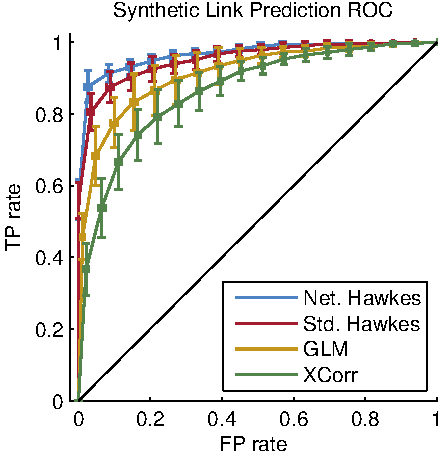
\includegraphics[width=\textwidth]{figures/ch2/synth_link_pred} 
    \label{fig:synth_link_pred}
  \end{subfigure}
  ~ ~ ~ ~
  \begin{subfigure}[T]{.4\textwidth}
    \caption{}
    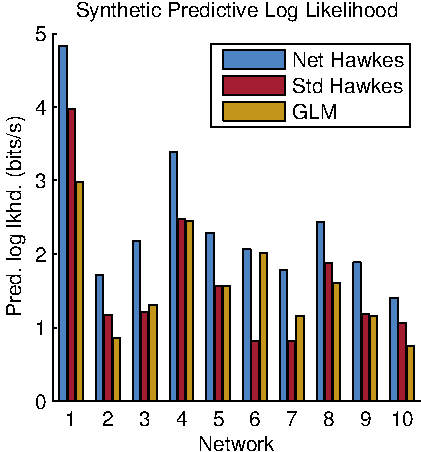
\includegraphics[width=\textwidth]{figures/ch2/synth_pred_ll}
    \label{fig:synth_pred_ll}
  \end{subfigure}
  \end{center}
  \vspace{-1em}
  \caption[Synthetic link prediction and predictive log likelihood]{
    \textbf{(a)} Comparison of models on a link prediction test
    averaged across ten randomly sampled synthetic networks of 30
    nodes each. The network Hawkes model with the correct
    Erd\H{o}s-Renyi graph prior outperforms a standard Hawkes model,
    GLM, and simple thresholding of the cross-correlation matrix.
    \textbf{(b)} Comparison of predictive log likelihoods, compared to
    a baseline of a Poisson process with constant rate. Improvement in
    predictive likelihood over baseline is normalized by the number of
    spikes in the test data to obtain units of ``bits per spike.'' The
    network Hawkes model outperforms the competitors in all sample
    networks.}
\end{figure}

We sampled ten network Hawkes processes of~$30$ nodes each with
Erd\H{o}s-Renyi graph models, constant background rates, and the
conjugate priors described above. The Hawkes
processes were simulated for~${T=1000}$ seconds. We used the models
above to predict the presence or absence of interactions. The results
of this experiment are shown in the ROC curves of
Figure~\ref{fig:synth_link_pred}. The network Hawkes model accurately
identifies the sparse interactions, outperforming all other models.
With the Hawkes process and the GLM we can evaluate the log likelihood
of held-out test data. On this task, the network Hawkes outperforms
the competitors for all networks. On average, the network Hawkes model
achieves~$2.2\pm.1$ bits/spike improvement in predictive log
likelihood over a homogeneous Poisson
process. Figure~\ref{fig:synth_pred_ll} shows that on average the
standard Hawkes and the GLM provide only 60\% and 72\%, respectively,
of this predictive power. See the supplementary material for further
analysis.

\section{Modeling Hippocampal Place Cells}

\begin{figure}[t]
  \begin{center}
  \begin{subfigure}[T]{1.4in}
    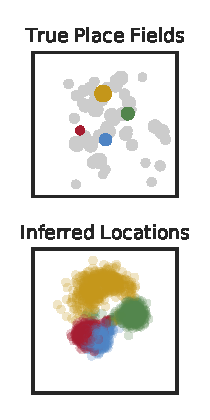
\includegraphics[width=\textwidth]{figures/ch2/locations_0} 
    \label{fig:hipp_locations_0}
  \end{subfigure}
  \begin{subfigure}[T]{1.4in}
    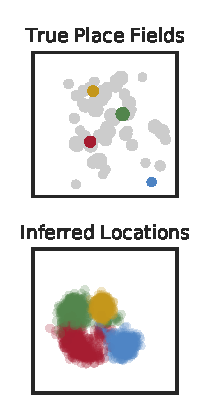
\includegraphics[width=\textwidth]{figures/ch2/locations_3} 
    \label{fig:hipp_locations_2}
  \end{subfigure}
  \begin{subfigure}[T]{1.4in}
    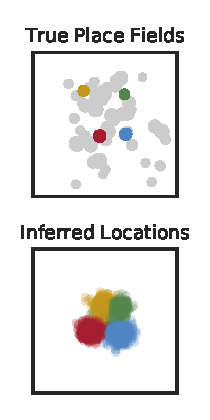
\includegraphics[width=\textwidth]{figures/ch2/locations_7} 
    \label{fig:hipp_locations_7}
  \end{subfigure}
  \begin{subfigure}[T]{1.4in}
    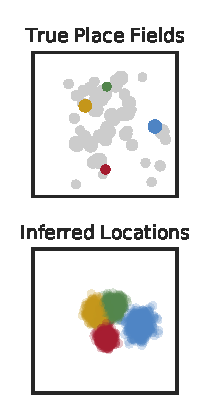
\includegraphics[width=\textwidth]{figures/ch2/locations_11} 
    \label{fig:hipp_locations_8}
  \end{subfigure}
  \vspace{-3em}
  \end{center}
  \caption[Inferred locations of hippocampal place cells]{ Inferred
    locations of hippocampal place cells using a latent distance model
    as a prior distribution over the adjacency matrix. For
    visualization, we show the posterior distribution over locations
    for four cells at a time.  \textbf{Top:} true place field
    centers. Marker size is proportional to the size of the place
    field. Larger dots imply less precise place fields, which should
    roughly translate to larger posterior variance over
    locations. \textbf{Bottom:} 250 samples from the posterior
    distribution over neuron locations for the four colored cells in
    the plot above. Each sample of locations (a~${49\times 2}$ matrix) is
    rotated to best match the true locations. Limits are the same in all plots.}
  \label{fig:hawkes_hipp}
\end{figure}

Our first real dataset consists of a simultaneously recorded
population of~$49$ hippocampal place cells from a rat freely foraging
in a circular arena roughly $120$cm in diameter. The data is courtesy
of the lab of Prof. Matthew Wilson at MIT. The recording duration was
roughly~$25$ minutes. The first~$20$ minutes were used for model fitting 
and the last~$5$ were reserved for predictive tests. Over the entire
$25$ minute recording, each neuron fired on average~$1979\pm4117$ spikes (min:~$48$,
max:~$27572$). This corresponds to a firing rate of~$1.35 \pm 2.82$Hz
(min:~$0.32$Hz, max:~$18.88$Hz). The rat's location,~$\bx(t)$, was recorded
along with the corresponding spike times. From this, the place field
of the~$n$-th neuron is computed as,
\begin{align*}
  \bar{\bx}_n &= \frac{1}{M_n} \sum_{m=1}^M \bx(s_m) \cdot \bbI[c_m=n],
\end{align*}
where, again,~$M_n$ is the number of spikes fired by neuron~$n$. Likewise,
the covariance of the place field is given by,
\begin{align*}
  \bV_n &= \left[ \frac{1}{M_n} \sum_{m=1}^M  \bx(s_m) \bx(s_m)^\trans  \cdot \bbI[c_m = n] \right] - \bar{\bx}_n \bar{\bx}_n^\trans.
\end{align*}
This gives us an estimate of the size of the place field. Let~${\bX= \{\bx_n\}}$
denote the~${49\times 2}$ matrix of place fields.

We compare a few different models for this data. Our baseline is a set
of independent Poisson processes with constant firing rates set by
maximum likelihood. Next, we consider a standard, densely connected
Hawkes process.  Third, we fit a network Hawkes process with an
independent Bernoulli prior on the adjacency matrix and an independent
gamma prior on the weight matrix. This induces sparsity in the
connectivity. Finally, we fit a network Hawkes model with a latent
distance prior on the adjacency matrix and an independent gamma prior
on the weights. In fitting this last model, we infer a distribution
over sets of locations,~${\bZ = \{\bz_n\}}$, for the population.


Intuitively, we expect these locations to mirror the true place fields
since nearby cells are likely to have correlated firing rates, which
should be captured by excitatory impulse responses between nearby
cells.  Figure~\ref{fig:hawkes_hipp} shows that this is indeed the
case.  In the top row, we plot the true place fields of the $49$
neurons.  The marker size is proportional to the size of the place
field, as measured by the largest eigenvalue of~$\bV_n$. Larger place
fields actually imply \emph{less} precise encodings of location, so we
expect these cells to be correlated with many others and hence also
more variability in the inferred neuron location.  Since the posterior
distribution over~$\bZ$ is difficult to visualize, we only show the
marginal distribution over four cell locations at a time.

The bottom row shows distributions for four sets of four cells each.
The colors match the corresponding neuron in the plot above. Since the
latent distance model is invariant to rotation, for each
sample~$\bZ^{(\ell)}$, we find the orthogonal matrix,~$\bR^{(\ell)}$,
that minimizes~${||\bX - \bR^{(\ell)} \bZ^{(\ell)}||_F}$ and apply it
to obtain a rotated set of locations,~${\widetilde{\bZ}^{(\ell)} =
  \bR^{(\ell)} \bZ^{(\ell)}}$.  Doing this for each sample yields a
set of locations~$\{\widetilde{\bZ}^{(\ell)}\}_{\ell=1}^L$. These
rotated sample are used to generate the scatter plots in the bottom
panels of Figure~\ref{fig:hawkes_hipp}.

Overall, the posterior distribution over locations is in close
correspondence with the true place fields. In some cases, neurons with
larger place fields (e.g. yellow neuron in left-most panels) have
considerably larger posterior variance than cells with smaller place
fields. With the exception of the gree and yellow neurons in the
second panel, the arrangement of the four cells also matches the
relative arrangement of the true place fields. This illustrates how
Hawkes processes combined with latent variable models can provide
interpretable portraits of complex datasets and find low-dimensional
embeddings that recover known structure.

\TODO{Table of predictive log likelihoods}



\section{Trades on the S\&P 100}
\label{sec:financial}

% Financial embedding
\begin{figure}[t]
  \vspace{-1em}
  \begin{center}
    \begin{subfigure}[T]{.75\textwidth}
      \centering
      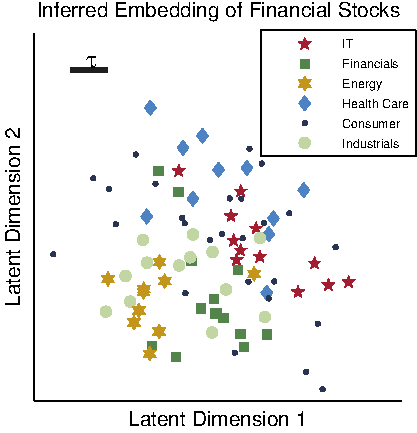
\includegraphics[width=.65\linewidth]{figures/ch2/financial_embedding} 
  \end{subfigure}
  \\
  \vskip1ex
  \begin{subfigure}[T]{.75\textwidth}
    \centering
    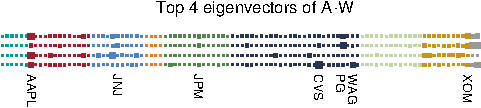
\includegraphics[width=\textwidth]{figures/ch2/financial_hinton} 
  \end{subfigure}
  \end{center}
  \vspace{-.5em}
  \caption[Financial embedding and dynamics eigenvectors]{
    \textbf{Top}: A sample from the posterior distribution over
    embeddings of stocks from the six largest sectors of the S\&P100
    under a latent distance graph model with two latent
    dimensions. Scale bar: the characteristic length scale of the
    latent distance model. The latent embedding tends to embed stocks
    such that they are nearby to, and hence more likely to interact
    with, others in their sector.
    \textbf{Bottom}: Hinton diagram of
    the top 4 eigenvectors. Size indicates magnitude of each stock's
    component in the eigenvector and colors denote sectors as in the
    top panel, with the addition of Materials (aqua), Utilities
    (orange), and Telecomm (gray). We show the eigenvectors
    corresponding to the four largest eigenvalues
    ${\lambda_{\mathsf{max}}=0.74}$ (top row) to ${\lambda_4=0.34}$
    (bottom row).}
  \label{fig:financial_embedding}
\end{figure}

While the focus of this thesis is on modeling \emph{neural}
spike trains, these models have broad applicability outside neuroscience
as well. Here we present one example in which we study the trades on the
S\&P~100 index collected at 1s intervals during the week of Sep.~28
through Oct.~2,~2009. Every time a stock price changes by~${\pm0.1\%}$
of its current price a spike is logged on the stock's process,
yielding a total of~${N=100}$ processes and~${M=182,037}$ spikes.

Trading volume varies substantially over the course of the day, with
peaks at the opening and closing of the market. Rather than attempting
to model this background fluctuation with a constant background rate,
here we use a log Gaussian Cox process (LGCP) with a periodic kernel
instead. Complete details of inference are given in
\citet{linderman2014discovering}. We look for short-term interactions
on top of this background rate with time scales of~${\Delta
  t_{\textsf{max}}=60\mathrm{s}}$.

In Figure~\ref{tab:financial_pred_ll} we compare the
predictive performance of independent LGCPs, a standard Hawkes process
with LGCP background rates, and the network Hawkes model with LGCP
background rates under two graph priors. The models are trained on
four days of data and tested on the fifth. Though the network Hawkes
is slightly outperformed by the standard Hawkes, the difference is
small relative to the performance improvement from considering
interactions, and the inferred network parameters provide
interpretable insight into the market structure.

In the latent distance model for~$\bA$, each stock has a latent
embedding~${\bx_k\in\reals^2}$ such that nearby stocks are more likely
to interact, as described in
Section~\ref{sec:graph_models}. Figure~\ref{fig:financial_embedding}
shows a sample from the posterior distribution over embeddings
in~$\reals^2$ for~${\rho=0.2}$ and~${\tau=1}$. We have plotted stocks
in the six largest sectors, as listed on Bloomberg.com. Some sectors,
notably energy and financials, tend to cluster together, indicating an
increased probability of interaction between stocks in the same
sector. Other sectors, such as consumer goods, are broadly
distributed, suggesting that these stocks are less influenced by
others in their sector. For the consumer industry, which is driven by
slowly varying factors like inventory, this may not be surprising.


% Table of financial results
\begin{table}
  \begin{center}
    \begin{tabular}{l|c}
      \textbf{Financial Model} & \textbf{Pred. log lkhd. (bits/spike)} \\
      \hline
      Independent LGCP & $0.594$ \\
      Standard Hawkes & $0.912$ \\
      Net. Hawkes ($\bA \sim $ Erd\H{o}s-Renyi Model) & $0.903$ \\
      Net. Hawkes ($\bA \sim $ Latent Distance Model) & $0.888$ \\
      %Net. Hawkes (SBM) & $0.894$ \\
    \end{tabular}
  \end{center}
    \caption{Comparison of financial models on a spike prediction task, relative to a homogeneous Poisson process baseline.}
    \label{tab:financial_pred_ll}
\end{table}


The Hinton diagram in the bottom panel of
Figure~\ref{fig:financial_embedding} shows the top $4$ eigenvectors of
the interaction network. All eigenvalues are less than $1$, indicating
that the system is stable. The top row corresponds to first
eigenvector~(${\lambda_{\mathsf{max}}=0.74}$). Apple~(\texttt{AAPL}),
J.P. Morgan~(\texttt{JPM}), and Exxon Mobil~(\texttt{XOM}) have
notably large entries in the eigenvector, suggesting that their
activity will spawn cascades of self-excitation.
% Removing this since it is entirely speculative
%The fourth eigenvector~(${\lambda_4=0.34}$) is dominated by Walgreens~(\texttt{WAG}) and CVS~(\texttt{CVS}), suggesting bursts of activity in these drug stores.
%, perhaps due to encouraging quarterly reports during flu season \cite{Walgreens-NYT-2009}.

\section{Gangs of Chicago}
\label{sec:chicago}
As a second example of applications outside neuroscience,
we study spatiotemporal patterns of gang-related
homicide in Chicago. Sociologists have suggested that gang-related
homicide is mediated by underlying social networks and occurs in
mutually-exciting, retaliatory patterns \cite{Papachristos-2009}. This
is consistent with a spatiotemporal Hawkes process in which processes
correspond to gang territories and homicides incite further homicides
in rival territories.

We study gang-related homicides between 1980 and 1995
\cite{ICPSR}. Homicides are labeled by the community in which they
occurred. Over this time-frame there were~${M=1637}$ gang-related
homicides in the~${77}$ communities of Chicago.

% Chicagoo results
\begin{figure}[!t]
  \begin{center}
    \begin{subfigure}[T]{.32\textwidth}
      \begin{subfigure}[T]{\textwidth}
        \begin{center}
          \caption{}
          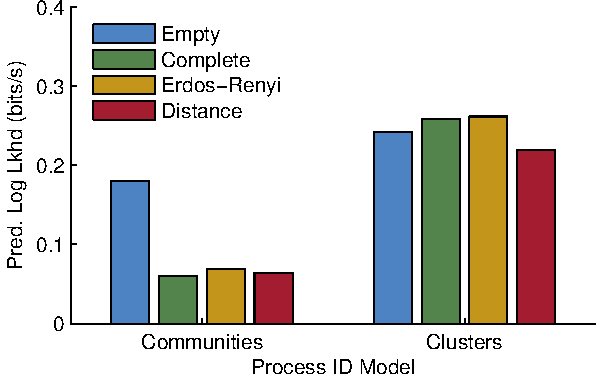
\includegraphics[width=\linewidth]{figures/ch2/icpsr_pred_ll}
          \label{fig:chicago_predll}
        \end{center}
      \end{subfigure}
      \begin{subfigure}[B]{\textwidth}
        \vspace{1em}
        \begin{center}
          \caption{}
          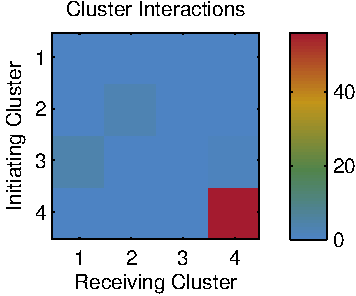
\includegraphics[width=.7\linewidth]{figures/ch2/icpsr_interactions}\\
          \label{fig:chicago_interactions}
        \end{center}
      \end{subfigure}
    \end{subfigure}
    ~
    \begin{subfigure}[B]{.32\textwidth}
      \caption{}
      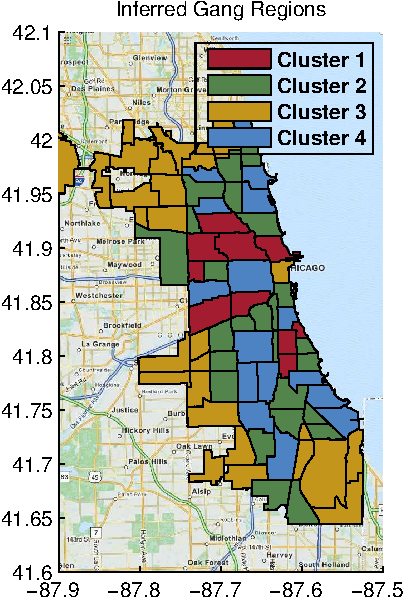
\includegraphics[width=\linewidth]{figures/ch2/icpsr_map} 
      \label{fig:chicago_map}
    \end{subfigure}
    \begin{subfigure}[B]{.28\textwidth}
      \caption{}
      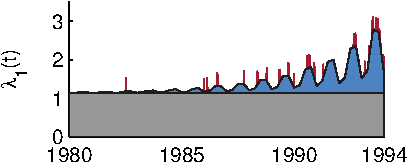
\includegraphics[width=\linewidth]{figures/ch2/icpsr_rate1} \\
      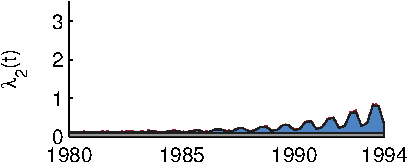
\includegraphics[width=\linewidth]{figures/ch2/icpsr_rate2} \\ 
      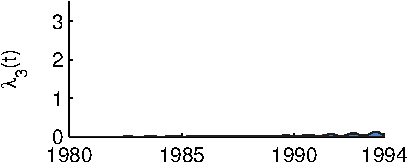
\includegraphics[width=\linewidth]{figures/ch2/icpsr_rate3} \\
      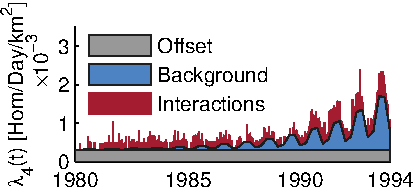
\includegraphics[width=\linewidth]{figures/ch2/icpsr_rate4} 
      \label{fig:chicago_rates}
    \end{subfigure}
  \end{center}
\vspace{-1em}
\caption[Inferred gang interactions in the city of Chicago]{
  Inferred interactions among clusters of community areas in the city of Chicago.
  \textbf{(a)} Predictive log likelihood for ``communities'' and ``clusters''  process identity models and four graph models. 
%Empty corresponds to independent LGCPs and Complete corresponds to the standard Hawkes process. 
  Panels \textbf{(b-d)} present results for the model with the highest predictive log likelihood: an Erd\H{o}s-Renyi graph with~${N=4}$ clusters.
  \textbf{(b)} The weighted interaction network in units of induced homicides over the training period (1980-1993).
  \textbf{(c)} Inferred clustering of the 77 community areas.
  \textbf{(d)} The intensity for each cluster, broken down into the offset, the shared background rate, and the interactions (units of~${10^{-3}}$ homicides per day per square kilometer).}
\label{fig:chicago}
\end{figure}


We evaluate our model with a spike-prediction task, training on
1980-1993 and testing on 1994-1995. We use a LGCP temporal background
rate in all model variations. Our baseline is a single process with a
uniform spatial rate for the city. Here, however, the analogous ``neurons''
are not so clear. We consider two models:  a)~the ``community'' model, which considers each community a separate ``neuron,'' or process, and b)~the ``cluster'' model, which groups
communities into processes. The number of clusters is chosen by
cross-validation (again, see \citet{linderman2014discovering}).
For each process identity model, we compare four graph models: a)~independent LGCPs
(\emph{empty}), b)~a standard Hawkes process with all possible
interactions (\emph{complete}), c)~a network Hawkes model with a
sparsity-inducing Erd\H{o}s-Renyi graph prior, and d)~a network Hawkes
model with a latent distance model that prefers short-range
interactions.

The community process identity model improves predictive performance
by accounting for higher rates in South and West Chicago where gangs
are deeply entrenched. Allowing for interactions between community
areas, however, results in a decrease in predictive power due to
overfitting (there is insufficient data to fit all~${77^2}$ potential
interactions). Interestingly, sparse graph priors do not help. They
bias the model toward sparser but stronger interactions which are not
supported by the test data. These results are shown in the
``communities'' group of Figure~\ref{fig:chicago_predll}. Clustering
the communities improves predictive performance for all graph models,
as seen in the ``clusters'' group. Moreover, the clustered models
benefit from the inclusion of excitatory interactions, with the
highest predictive log likelihoods coming from a four-cluster
Erd\H{o}s-Renyi graph model with interactions shown in
Figure~\ref{fig:chicago_interactions}. Distance-dependent graph priors
do not improve predictive performance on this dataset, suggesting that
either interactions do not occur over short distances, or that local
rivalries are not substantial enough to be discovered in our
dataset. More data is necessary to conclusively say which.

Looking into the inferred clusters in Figure~\ref{fig:chicago_map} and
their rates in~\ref{fig:chicago_rates}, we can interpret the clusters
as ``safe suburbs'' in gold, ``buffer neighborhoods'' in green, and
``gang territories'' in red and blue. Self-excitation in the blue
cluster (Figure~\ref{fig:chicago_interactions}) suggests that these
regions are prone to bursts of activity, as one might expect during a
turf-war. This interpretation is supported by reports of ``a burst of
street-gang violence in 1990 and 1991'' in West Englewood
(${41.77^\circ}$N, ${-87.67^\circ}$W) \cite{Block-1993}.

Figure~\ref{fig:chicago_rates} also shows a significant increase in
the homicide rate between 1989 and 1995, consistent with reports of
escalating gang warfare \cite{Block-1993}. In addition to this
long-term trend, homicide rates show a pronounced seasonal effect,
peaking in the summer and tapering in the winter. A LGCP with a
quadratic kernel point-wise added to a periodic kernel captures both
effects.

\section{Discussion}
Hawkes processes and latent network discovery have been a subject
of recent interest in the machine learning community. Much of this
interest stems from the growth of social networking applications
which produce massive amounts of spiking data. 
\citet{Gomez-2010} introduced one of the earliest algorithms for
discovering latent networks from cascades of spikes in social network
data. They developed a
highly scalable approximate inference algorithm, but they did not
explore the potential of random network models or emphasize the point
process nature of the data.
\citet{Simma-2010} studied this problem from the context of Hawkes
processes and developed an expectation-maximization inference
algorithm that could scale to massive datasets, like the interactions
between authors on Wikipedia.
We have adapted their latent variable formulation in our
fully-Bayesian inference algorithm and introduced a framework for
prior distributions over the latent network.

Others have considered special cases of the model we have
proposed. \citet{Blundell-2012} combine Hawkes processes and the
Infinite Relational Model (a specific exchangeable graph model with an
Aldous-Hoover representation) to cluster processes and discover
interactions in email networks. \citet{Cho-2013} applied Hawkes processes to gang
incidents in Los Angeles. They developed a spatial Gaussian mixture
model (GMM) for process identities, but did not explore structured
network priors. We experimented with this process identity model but
found that it suffers in predictive log likelihood tests.

Recently, \citet{Iwata-2013} developed a stochastic EM algorithm for
Hawkes processes, leveraging similar conjugacy properties, but without
network priors. \citet{Zhou-2013} have developed a promising
optimization-based approach to discovering low-rank networks in Hawkes
processes, similar to some of the network models we explored.

\citet{Perry-2013} derived a partial likelihood inference algorithm
for Hawkes processes with a similar emphasis on structural patterns in
the network of interactions. They provide an estimator capable of
discovering homophily
and other network effects. Our fully-Bayesian approach generalizes
this method to capitalize on recent developments in random network
models \cite{Lloyd-2012}.

Finally, generalized linear models (GLMs) are widely used in
computational neuroscience \cite{Paninski-2004}. GLMs allow for both
excitatory and inhibitory interactions, but, as we have shown, when
the data consists of purely excitatory interactions, Hawkes processes
outperform GLMs in link- and spike-prediction tests. We will discuss
these models in Chapter~\ref{chap:five}

This chapter developed a framework for discovering latent network
structure from spiking data with mutually excitatory interactions. Our
auxiliary variable formulation of the multivariate Hawkes process
supports a broad class of prior distributions on latent network
structure. This allows us to connect interpretable latent variables,
like neuron types and features, to a dynamic model for spike trains.
Our parallel MCMC algorithm allowed us to reason about uncertainty in
the latent network in a fully-Bayesian manner.  We leveraged results
from random matrix theory to analyze the conditions under which random
network models will be stable, and our applications uncovered
interpretable latent networks in a variety of synthetic and real-world
problems.

Hawkes processes are the point process analogue of linear autoregressive
models. The firing rate is a sum of non-negative impulse responses induced
by preceding spikes. As we generalize these models in the following
chapters, we will exploit this relationship and consider natural extensions
like discrete time, nonlinear, and nonstationary versions of the model.



